\chapter{Preliminaries}

Designing an effective Discrete Event Simulation (DES) system requires a solid understanding of the fundamental concepts underpinning parallel and distributed simulation systems \cite{PaDSS}.

Simulation, at its core, involves creating a model that captures the behavior of a real-world system over time. Such a system is characterized by a set of states that evolve dynamically in response to events. To accurately simulate a physical system, three essential criteria must be met:

\begin{enumerate}
    \item \textbf{Representation of the System State}: A mechanism to define and maintain the system's state variables.
    \item \textbf{Mechanism for State Evolution}: A way to modify the state to reflect changes over time, typically triggered by the occurrence of discrete events.
    \item \textbf{Abstraction of Time}: A logical construct for time that allows the simulation to progress through events, preserving temporal relationships.
\end{enumerate}

In computer simulations, the system state is represented using a set of state variables, which are updated according to the simulated progression of the system. These state variables are usually expressed in high-level programming languages such as C++ or Java. Time is modeled using an abstraction known as \textit{simulation time}, which will be discussed in detail in the subsequent sections.

\section{Concepts of Time}

A robust understanding of the various notions of time is essential for creating effective simulation models. The primary time concepts relevant to simulations include:

\begin{itemize}
    \item \textbf{Physical Time}: The actual time in the real-world system being simulated.
    \item \textbf{Simulation Time}: An abstraction used to model the physical time within the simulation environment.
    \item \textbf{Real Time}: The actual elapsed time during the execution of the simulation, typically measured using the hardware clock of the underlying operating system.
\end{itemize}

\subsection{Formal Definition of Simulation Time}

Simulation time is formally defined as a totally ordered set of values, where each value represents a specific temporal instant within the simulated system. For two simulation time values, $T_1$ and $T_2$, if $T_1 < T_2$, it signifies that the event corresponding to $T_1$ occurs before the event corresponding to $T_2$. This ordering of simulation time values ensures that temporal relationships among events are preserved within the simulation environment.

\section{Modes of Execution}

Simulations can be executed in different modes depending on how simulation time progresses relative to real time:

\begin{itemize}
    \item \textbf{Real-Time Execution}: The simulation time advances at the same rate as real time, ensuring that simulated events occur synchronously with real-world events.
    \item \textbf{Scaled Real-Time Execution}: The progression of simulation time is governed by a constant scaling factor, allowing it to run faster or slower than real time. For example, a scaling factor of 2 means that every second of real time corresponds to two seconds of simulated time.
    \item \textbf{As-Fast-As-Possible Execution}: The simulation progresses as quickly as possible, unconstrained by real time. This mode is ideal for scenarios that require multiple iterations, as it allows the simulation to complete in the shortest possible duration.
\end{itemize}

\section{Discrete-Event Simulation}

Discrete-event simulation (DES) is characterized by updating the state of the system only when specific events occur. An event is defined as an instantaneous change in the system's state and is associated with a timestamp that indicates its occurrence in simulation time. The simulation advances by processing events in chronological order, updating state variables only when necessary.

\begin{algorithm}[H]
\caption{Discrete-Event Simulation Based on Real-Time Execution} \label{alg:client_simulation}
\begin{algorithmic}[1]
    \STATE \textbf{Initialize} simulation parameters and state variables.
    \WHILE{simulation is running}
        \STATE Wait until \texttt{W2S} (real time) $\geq$ simulation time.
        \STATE Compute the system's state at the end of this interval.
        \STATE Advance simulation time to the next event time.
    \ENDWHILE
\end{algorithmic}
\end{algorithm}

Unlike continuous simulations, where time progresses in fixed intervals, DES jumps from one event to the next, skipping periods where no state changes occur. This event-driven approach enhances efficiency by minimizing unnecessary state computations.

\begin{figure}[H]
    \centering
    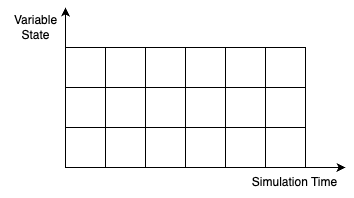
\includegraphics[width=0.7\textwidth]{images/constTime.png}
    \caption{Space-Time Diagram for Time-Stepped Simulation}
    \label{fig:constTime}
\end{figure}

\begin{figure}[H]
    \centering
    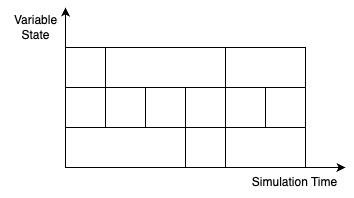
\includegraphics[width=0.7\textwidth]{images/sparseTime.png}
    \caption{Space-Time Diagram for Event-Driven Simulation}
    \label{fig:sparseTime}
\end{figure}

In scenarios where real-time consistency is required, discrete-event simulations can be synchronized to ensure that simulation time progresses in lockstep with real time. This synchronization enables a more cohesive and accurate representation of real-world processes.

\section{Discrete-Event Simulation Framework}

The focus of this work is on discrete-event simulations. A typical DES program relies on three fundamental data structures:

\begin{enumerate}
    \item \textbf{State Variables}: These variables represent the current state of the system.
    \item \textbf{Event List}: A priority queue containing events scheduled to occur at future simulation times, each with a corresponding timestamp.
    \item \textbf{Global Clock Variable}: Represents the current simulation time. If the clock variable has a value $T$, it indicates that all activities up to time $T$ have been simulated, while activities beyond $T$ are yet to be processed.
\end{enumerate}

An event in the DES framework typically consists of a data structure containing its timestamp (e.g., 9:16 AM), event type (e.g., airplane arrival), and various parameters specifying details of the event (e.g., Flight 396 arriving at LAX).

In a physical system, events such as airplane arrivals occur autonomously. In the simulation, however, nothing happens unless an event is explicitly created by the simulation computation. This process is referred to as \textit{event scheduling}. For example, if the simulation reaches time 9:00 and an event indicates that Flight 200 has landed, the simulation can then schedule a new event for this plane’s departure at 9:56. Event scheduling involves allocating memory for a new event, populating its fields (timestamp, event type, and parameters), and adding it to the event list.

\begin{figure}[H]
    \centering
    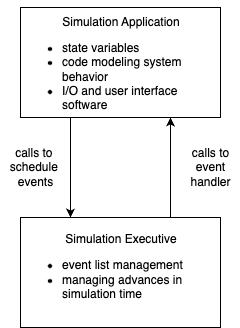
\includegraphics[width=0.4\textwidth]{images/simulationComponents.png}
    \caption{Separation of the Simulation Program into the Simulation Application and Executive Components}
    \label{fig:simComp}
\end{figure}

A discrete-event simulation program can be divided into two major components, as illustrated in Figure~\ref{fig:simComp}:

\begin{itemize}
    \item \textbf{Simulation Executive}: This component maintains the event list and the global clock variable. It operates independently of the specific physical system being simulated, serving as the backbone of the simulation program. Often, it is provided as a generic software library adaptable to simulate various types of systems.
    \item \textbf{Simulation Application}: This component contains the state variables and software routines for modeling the physical system. It is closely tied to the specific characteristics and behaviors of the real-world system being simulated. In its simplest form, the simulation executive must only provide one primitive procedure to the simulation application: a method for scheduling events.
\end{itemize}

The core of the simulation executive is an event-processing loop that repeatedly removes the event with the smallest timestamp from the event list, simulates its occurrence, and advances the simulation clock.
